% !TeX root = ../tfg.tex
% !TeX encoding = utf8

\chapter{Teoría de la Probabilidad}\label{ch:capitulo-teoria-de-la-probabilidad}

En este capítulo se presentarán definiciones y resultados fundamentales de la teoría de la probabilidad y la estadística, con el propósito de introducir conceptos clave que faciliten la comprensión del fenómeno y que utilizaremos a lo largo del desarrollo de gran parte del trabajo. Las fuentes principales utilizadas a lo largo de este capítulo son extractos de~\cite{Dembo2014} y~\cite{Knill2009}.\newline

\section{Espacios de probabilidad y $\sigma$-álgebras}

Para establecer la base teórica, consideraremos un conjunto arbitrario $\Omega$, al que nos referiremos como \emph{espacio muestral} y que representa el conjunto de todos los posibles resultados al realizar un experimento. Asimismo, llamaremos \emph{suceso} a cualquier subconjunto de $\Omega$.\newline

\begin{definicion}[\emph{$\sigma$-álgebra}]\label{def:sigma-algebra}
    Un conjunto $\mathcal{A}$ de subconjuntos de $\Omega$ ($\mathcal{A} \subseteq \mathcal{P}(\mathcal{A})$) se dirá que es una \emph{$\sigma$-álgebra} si verifica las siguientes propiedades:

    \begin{itemize}
        \item $\Omega \in \mathcal{A}$,
        \item Si $\mathrm{A} \in \mathcal{A}$, entonces $\mathrm{A}^c = \Omega \setminus \mathcal{A} \in \mathcal{A}$ ($\mathrm{A}$ es cerrado bajo complementarios),
        \item Si $\mathrm{A}_{n} \in \mathcal{A}$, entonces $\bigcup_{n \in \mathbb{N}} \mathrm{A}_{n} \in \mathcal{A}$ (A es cerrado bajo uniones finitas)
    \end{itemize}
\end{definicion}

Es fácil comprobar que $\mathcal{A}$ es cerrado bajo intersecciones finitas y que, además, la intersección de $\sigma$-álgebras es una $\sigma$-álgebra.\newline

\begin{definicion}[\emph{$\sigma$-álgebra de Borel}]\label{def:sigma-algebra-borel}
    Para cada conjunto $\mathcal{C}$ de subconjuntos de $\Omega$, se define $\sigma(\mathcal{C})$ como la menor $\sigma$-álgebra $\mathcal{A}$ que contiene a C. La $\sigma$-álgebra $\mathcal{A}$ es la intersección de todas las $\sigma$-álgebras que contienen a C y, por tanto, es una $\sigma$-álgebra.

    Si ($\mathrm{E}, \mathcal{O}$) es un espacio topológico, donde $\mathrm{O}$ es el conjunto formado por los conjuntos abiertos en E, entonces $\sigma(\mathcal{O})$ es llamada la \textbf{$\sigma$-álgebra de Borel} del espacio topológico.
\end{definicion}

Llamaremos \emph{espacio de medida} al conjunto ($\Omega, \mathcal{A}$) donde $\mathcal{A}$ es una $\sigma$-álgebra en $\Omega$.\newline

\begin{definicion}[\emph{Medida de probabilidad}]\label{def:medida-de-probabilidad}
    Dado un espacio de medida ($\Omega, \mathcal{A}$), una función $\mathrm{P}: \mathcal{A} \to \mathbb{R}$ se llamará \emph{medida de probabilidad} si cumple las siguientes tres propiedades (conocidas como \textbf{axiomas de Kolmogorov}~\cite{Kolmogorov1956}):

    \begin{itemize}
        \item $\mathrm{P}[\mathrm{A}] \ge 0$ para todo $\mathrm{A} \in \mathcal{A}$,
        \item $\mathrm{P}[\Omega]=1$,
        \item $\mathrm{P}$ es $\sigma$-aditiva, es decir, si $\mathrm{A}_n \in \mathcal{A}$ con $n \in \mathbb{N}$ son conjuntos disjuntos dos a dos, entonces 
        \[ \mathrm{P}\left[\bigcup_{n \in \mathbb{N}} \mathrm{A}_{n}\right] = \sum\limits_{n \in \mathbb{N}} \mathrm{P}[\mathrm{A}_n]. \]
    \end{itemize}
\end{definicion}

La primera condición nos asegura la no negatividad de la probabilidad, es decir, la probabilidad nunca será inferior a $0$. A su vez, la segunda condición nos establece que la probabilidad del espacio muestral completo ($\Omega$) debe ser igual a 1, es decir, refleja que uno de los eventos posibles siempre ocurrirá, conocido como \emph{suceso seguro}.\newline

\begin{observacion}
Dado que una medida de probabilidad es, por definición, una \emph{medida}, se sigue de manera inmediata que $\mathrm{P}(\emptyset) = 0$. Además, al conjunto $\emptyset$ se le suele denotar como \emph{evento imposible}.\newline
\end{observacion}

\begin{corolario}\label{cor:propiedades-adicionales}
    Algunas propiedades básicas de la medida de probabilidad ($\mathrm{P}$) que se siguen de la propia definición son las siguientes:

    \begin{enumerate}
        \item Si $\mathrm{A}, \mathrm{B} \in \mathcal{A}$ y $\mathrm{A} \subset B$, entonces $\mathrm{P}[\mathrm{A}] \le \mathrm{P}[\mathrm{B}]$.
        \item $\mathrm{P}[\mathrm{A^c}] = 1-\mathrm{P}[\mathrm{A}]$, para todo $\mathrm{A} \in \mathcal{A}$.
        \item $0 \le \mathrm{P}[\mathrm{A}] \le 1$ para todo $\mathrm{A} \in \mathcal{A}$.\newline
    \end{enumerate}
\end{corolario}

\begin{observacion}
Existen distintas formas de construir los axiomas para un espacio de probabilidad. Por ejemplo, se podrían sustituir las primeras dos propiedades de la definición de medida de probabilidad por las últimas dos propiedades enunciadas en el corolario anterior.\newline
\end{observacion}

\begin{definicion}[\emph{Espacio de probabilidad}]\label{def:espacio-de-probabilidad}
    Dado un espacio de medida ($\Omega, \mathcal{A}$), llamaremos \emph{espacio de probabilidad} a la tripleta ($\Omega, \mathcal{A}, \mathrm{P}$), donde $\mathrm{P}$ es una medida de probabilidad.\newline
\end{definicion}

\section{Variables aleatorias y esperanza}

Las variables aleatorias son funciones numéricas que asignan un valor numérico a cada posible resultado de un experimento aleatorio $w \in \Omega$. De manera intuitiva, una variable aleatoria puede verse como una cantidad numérica cuyo valor no es fijo y que puede tomar distintos valores, por lo que es necesario definir una distribución de probabilidad que asocie probabilidades a los distintos valores que pueda tomar la variable aleatoria. \newline

\begin{definicion}[\emph{Función medible}]\label{def:funcion-medible}
    Una función $X: (\Omega_1, \mathcal{A}) \to (\Omega_2, \mathcal{B})$ se dice \emph{medible} si

    \[ X^{-1}(\mathrm{B}) \in \mathcal{A} \quad \forall \, \mathrm{B}  \in \mathcal{B} \]

    donde el conjunto $ X^{-1}(\mathrm{B})$ se encuentra formado por todos los puntos $x \in \Omega$ para los cuales $X(x) \in \mathrm{B}$.\newline
\end{definicion}

\begin{definicion}[\emph{Variable aleatoria}]\label{def:variable-aleatoria}
    Dado un espacio de probabilidad ($\Omega_1, \mathcal{A}, \mathrm{P}$) y un espacio medible ($\Omega_2, \mathcal{B}$), decimos que $X: (\Omega_1, \mathcal{A}, \mathrm{P}) \to (\Omega_2, \mathcal{B})$ es una \emph{variable aleatoria} si $X$ es una función medible.
\end{definicion}

Además, si el espacio medible de llegada es $n$-dimensional, entonces la variable aleatoria $X$ es llamada \textit{vector aleatorio} y lo denotaremos por $X = (X_1, X_2, \ldots, X_n)$ donde cada componente $X_i$ con $i \in \{1, 2, \ldots, n\}$ es una variable aleatoria.\newline

\begin{observacion}
    En la mayoría de usos prácticos se tiene que el espacio medible de llegada más común es ($\mathbb{R}, \mathcal{B}(\mathbb{R})$), donde $\mathcal{B}(\mathbb{R})$ denota la $\sigma$-álgebra de Borel en $\mathbb{R}$.\newline
\end{observacion}

\begin{definicion}
    Diremos que una variable aleatoria es \emph{discreta} si esta toma un número finito o numerable de valores en el espacio de llegada. Por otra parte, si la variable aleatoria toma un número infinito o no numerable de valores, diremos que es una variable aleatoria \emph{continua}.\newline
\end{definicion}

\begin{ejemplo}
    Como ejemplo sencillo podemos considerar los posibles resultados obtenidos al lanzar un dado de seis caras, es decir, $w \in \{1,2,3,4,5,6\}$ y podemos definir la variable aleatoria discreta que asigna el valor de la cara superior del dado cuando se lanza. En este caso, la variable aleatoria se define como:

    \[ X(w) = w \quad para \, w \in \{1,2,3,4,5,6\}. \]\newline
\end{ejemplo}

\begin{definicion}[Función de distribución]\label{def:funcion-de-distribucion}
    La función de distribución (acumulada) de una variable aleatoria $X$ es una función $F_X: \mathbb{R} \to [0,1]$ dada por

    \[ F_X(\alpha) = P[\{ w:X(w) \le \alpha\}] \quad \forall \alpha \in \mathbb{R}. \]\newline
\end{definicion}

\begin{proposicion}
    La función de distribución $F$ de una variable aleatoria $X$ cumple las siguientes propiedades:

    \begin{enumerate}
        \item $F$ es monótona no decreciente.
        \item $\lim_{x \to \infty} F(x) = 1$ y $\lim_{x \to -\infty} F(x) = 0$.
        \item $F$ es continua por la derecha, es decir, $\lim_{y \to x^+} F(y) = F(x)$.\newline
    \end{enumerate}
\end{proposicion}

\begin{definicion}[Función de probabilidad]\label{def:funcion-de-probabilidad}
    Sea $X$ una variable aleatoria discreta, llamaremos \emph{función (masa) de probabilidad}, a la función que asigna la probabilidad de que la variable aleatoria tome un valor en particular, es decir:

    \[ p_X(x) = P[X = x] \quad donde \; x \in \{x_1, \ldots, x_n\}. \]
\end{definicion}

Las probabilidades asociadas con todos los posibles resultados del experimento deben ser no negativas y sumar $1$, es decir $ \sum_x p_X(x) = 1 $ y, además, $p_X(x) \ge 0$.\newline

Notemos que, el concepto de función de probabilidad, solo tiene sentido al hablar de variables aleatorias discretas. Para variables aleatorias continuas, el concepto análogo es el de función de densidad, donde deberemos integrar para obtener la probabilidad, pues la probabilidad asociada a un único punto en un intervalo es cero.\newline

\begin{definicion}[Función de densidad]\label{def:funcion-de-densidad}
    Se dice que una función $f_X$ integrable de Lebesgue, no negativa en casi todas partes es la \emph{función de densidad} de una variable aleatoria continua $X$ si su función de distribución puede ser expresada como

    \[ F_X(\alpha) =  \int_{-\infty}^{\alpha} f_X(x) \, dx \quad \forall \alpha \in \mathbb{R}. \]
\end{definicion}

Notemos que la función de densidad, de manera análoga a la función de probabilidad, cumple $ f_X(x) \ge 0$ y $ \int_{-\infty}^{\infty} f_X(x) = 1$.\newline

\begin{definicion}[Esperanza de una variable aleatoria]\label{def:esperanza-variable-aleatoria}
Sea $X$ una variable aleatoria en el espacio de probabilidad ($\Omega, \mathcal{A}, \mathrm{P}$). Definimos la \emph{esperanza o valor esperado} de $X$, denotado por $E[X]$ como la integral de Lebesgue siguiente:

\[ \mathbb{E}[X] = \int_{\Omega} X(w)dP[w]. \]

Para vectores aleatorios, su esperanza viene definida componente a componente:

\[ \mathbb{E}[(X_1, \ldots, X_n)] = (\mathbb{E}[X_1], \ldots, \mathbb{E}[X_n]). \]\newline
\end{definicion}

\begin{observacion}
    Si $X$ es una variable aleatoria discreta con función de probabilidad $\mathrm{P}[X = x_i]$ con $i \in \{1,2,\ldots,n\}$, su esperanza viene definida por:

    \[ \mathbb{E}[X] = \sum_{i=1}^{n} x_i \: \mathrm{P}[X = x_i]. \]

    donde $x_i$ denota cada posible resultado del experimento.\newline
\end{observacion}

\begin{observacion}
    Si $X$ es una variable aleatoria continua con función de densidad $f_X(x)$, su esperanza viene definida por:

    \[ \mathbb{E}[X] =  \int_{\mathbb{R}} x \;f_X(x) \, dx. \]\newline
\end{observacion}

\subsection{Probabilidad condicional}

En esta sección introduciremos la noción clásica de \emph{probabilidad condicional} de sucesos, ligada al supuesto de conocer la probabilidad de un cierto suceso bajo la condición de que ocurra otro suceso. De igual manera, se introducirán resultados necesarios para el desarrollo del trabajo, tales como el teorema de Bayes.\newline

\begin{definicion}\label{def:probabilidad-condicional}
    Dados dos sucesos $A, B \in \mathcal{A}$ con $P[B] > 0$, definimos la \emph{probabilidad condicional} de $A$ con respecto a $B$ de la siguiente forma:

    \[ P[A|B] = \frac{P[A \cap B]}{P[B]}. \]\newline
\end{definicion}

\begin{definicion}\label{def:particion-finita}
    Un conjunto finito $\{A_1, \ldots, A_n \} \subset \mathcal{A}$ se denominará \emph{partición finita} de $\Omega$ si cumple:

    \begin{enumerate}
        \item $\bigcup\limits_{i=1}^n A_i = \Omega$.
        \item $A_i \cap A_j = \emptyset$ para todo $i \neq j$.
    \end{enumerate}
\end{definicion}

Una partición finita cubre todo el espacio con un número finito de conjuntos (sucesos) disjuntos dos a dos.\newline

\begin{teorema}[Probabilidad total]\label{teo:probabilidad-total}
    Sean $\{A_1, \ldots, A_n \}$ una partición finita de $\mathcal{A}$ y $B \in \mathcal{A}$ un suceso cualquiera del que se conocen las probabilidades condicionales $P[B|A_i] \; \forall \, i \in \{1, \ldots, n \}$, entonces la probabilidad del suceso $B$ viene dada por la siguiente expresión:

    \[ P[B] = \sum_{i=1}^{n} P[B|A_i]P[A_i]. \]\newline
\end{teorema}

\begin{proof}
    Partimos de una partición finita $\{A_1, \ldots, A_n \}$ de $\mathcal{A}$ y de un suceso $B \in \mathcal{A}$. Usando la primera propiedad de la Definición~\ref{def:particion-finita}, podemos expresar el suceso B de la siguiente forma:

    \[ B = (B \cap A_1) \cup (B \cap A_2) \cup \ldots \cup (B \cap A_n). \]\newline

    Usando la segunda propiedad de la Definición~\ref{def:particion-finita}, sabemos que $A_i \cap A_j = \emptyset, i \neq j$. Por tanto, obtenemos que los conjuntos $(B \cap A_i), \; i \in \{1, \ldots, n\}$ son, también, disjuntos dos a dos.\newline

    Por consiguiente, podemos expresar la probabilidad del suceso $B$ como sigue:

    \[ P[B] = P[B \cap A_1] + P[B \cap A_2] + \cdots + P[B \cap A_n]. \]\newline

    Finalmente, usando la Definición~\ref{def:probabilidad-condicional}, obtenemos que 
    \[ P[A_i \cap B] = P[A_i | B]P[B],\; \forall \; i \in \{1, \ldots, n\}. \]\newline
    
    Por tanto, obtenemos la expresión buscada:
    \begin{align*}
        P[B] &= P[B \cap A_1] + P[B \cap A_2] + \cdots + P[B \cap A_n] \\
             &= P[B|A_1]P[A_1] + P[B|A_2]P[A_2] + \cdots + P[B|A_n]P[A_n] \\
             &= \sum_{i=1}^n P[B|A_i]P[A_i].
    \end{align*}
\end{proof}

Llegados a este punto estamos en las condiciones necesarias de introducir un teorema fundamental que nos permite calcular probabilidades condicionales. Este resultado vincula la probabilidad de un suceso $A$ dado otro suceso $B$ ($P[A|B]$) con la probabilidad del suceso $B$ dado el suceso $A$ ($P[B|A]$).\newline

\begin{teorema}[Regla de Bayes]\label{teo:teorema-de-bayes}
    Dada una partición finita $\{A_1, \ldots, A_n \}$ de $\mathcal{A}$ y un suceso $B \in \mathcal{A}$ con $P[B] > 0$, se verifica:

    \[ P[A_i | B] = \frac{P[B | A_i]P[A_i]}{\sum_{i=1}^n P[B|A_i]P[A_i]}. \]\newline
\end{teorema}

\begin{proof}
    En primer lugar, de la Definición~\ref{def:probabilidad-condicional}, sabemos que
     $P[A_i|B] = \frac{P[A_i \cap B]}{P[B]}$. Además, del Teorema~\ref{teo:probabilidad-total}, conocemos que $P[B] = \sum_{i=1}^n P[B|A_i]P[A_i]$.\newline

    Por otra parte, aplicando la Definición~\ref{def:probabilidad-condicional} de la siguiente manera:

    \[ P[B|A_i] = \frac{P[B \cap A_i]}{P[A_i]}. \]\newline

    Ahora, despejando, obtenemos $P[A_i \cap B] = P[B \cap A_i] = P[B|A_i]{P[A_i]}$. Finalmente, combinado ambos resultados alcanzamos la conclusión buscada:

    \[ P[A_i|B] = \frac{P[A_i \cap B]}{P[B]} = \frac{P[B | A_i]P[A_i]}{\sum_{i=1}^n P[B|A_i]P[A_i]}. \]
    
\end{proof}

\subsection{Independencia de variables aleatorias}

En esta sección nos centraremos en explicar el concepto de independencia en el contexto de las variables aleatorias. De manera intuitiva, el concepto de independencia, como su nombre indica, va ligado al hecho de que el conocimiento que poseamos de una de las variables no proporciona información adicional sobre el conocimiento de la otra. Para ello, también expandiremos el concepto de función de distribución para el caso de más de una variable aleatoria (vector aleatorio).\newline

\begin{definicion}[Función de distribución conjunta]\label{def:funcion-de-distribucion-conjunta}
    Sean $X_1, \ldots, X_n$ variables aleatorias definidas sobre el mismo espacio de probabilidad $(\Omega, \mathcal{A}, \mathrm{P})$, la \emph{función de distribución conjunta} es una función $F_{X_{1}, \ldots, X_{n}}: \mathbb{R} \to [0,1]$ dada por

    \[ F_{X_{1}, \ldots, X_{n}}(x_1, \ldots, x_n) = P[X_1 \leq x_1, \ldots, X_n \leq x_n], \quad x_1, \ldots, x_n \in \mathbb{R}. \]

    Si interpretamos las n variables aleatorias como un vector aleatorio $X = (X_1, \ldots, X_n)$, podemos simplificar la notación de la siguiente forma:

    \[ F_{X_{1}, \ldots, X_{n}}(x_1, \ldots, x_n) = F_X(x_1, \ldots, x_n). \]\newline
\end{definicion}

De la misma forma, podemos extender las definiciones de \emph{función de probabilidad} y \emph{función de densidad} para el caso en el que dispongamos de más de una variable aleatoria.\newline

En primer lugar, comenzaremos definiendo y demostrando el resultado de la \emph{regla de la cadena} para probabilidades que nos será de gran utilidad para trabajar con las siguientes definiciones.\newline

\begin{teorema}[Regla de la cadena]
    Sea ($\Omega, \mathcal{A}, P$) un espacio de probabilidad y $\{A_1, \ldots, A_n \} \in \mathcal{A}$ una serie de sucesos. Entonces, se verifica

    \[ P[A_1 \cap A_2 \cap \ \ldots \ \cap A_n] =  P[A_1]P[A_2 | A_1]\cdots \ P[A_1]\prod_{i=2}^n P[A_i | A_1 \ \cap \cdots \ \cap A_{i-1}]. \]\newline
\end{teorema}

\begin{proof}
    La demostración se realiza de manera sencilla por recursión teniendo en cuenta que en el primer caso se hace uso de la Definición~\ref{def:probabilidad-condicional}:

    \[ P[A_1 \cap A_2] = P[A_1]P[A_2| A_1]. \]\newline
\end{proof}

\begin{definicion}[Función de probabilidad conjunta]
    Sean $X_1, \ldots, X_n$ variables aleatorias discretas. La \emph{función (masa) de probabilidad conjunta} de dichas variables viene dada por

    \[ p_{X_1, \ldots, X_n}(x_1, \ldots, x_n) = P(X_1 = x_1, \ldots, X_n = x_n), \quad (x_1, \ldots, x_n) \in \mathbb{R}^n. \]

    Equivalentemente, la función de probabilidad conjunta puede ser expresada de la siguiente forma:

    \begin{align*}
        p_{X_1, \dots, X_n}(x_1, \dots, x_n) &= P(X_1 = x_1) \cdot P(X_2 = x_2 \mid X_1 = x_1) \cdot \\
        &\quad \cdot P(X_3 = x_3 \mid X_1 = x_1, X_2 = x_2) \cdots \\
        &\quad \cdot P(X_n = x_n \mid X_1 = x_1, X_2 = x_2, \dots, X_{n-1} = x_{n-1})
    \end{align*}

    donde se utiliza la definición de probabilidad condicionada y la regla de la cadena comentada en el teorema anterior.\newline
\end{definicion}

Además, dado que estamos trabajando con probabilidades, se verifica que la suma total debe ser igual a 1, es decir 
\[ \sum_{i}\sum_{j}\ldots\sum_{k}P[X_1=x_{1i}, X_2=x_{2j}, \ldots, X_n=x_{nk}] \]
donde los distintos índices ($i, j, \ldots, k$) recorren todos los posibles resultados de cada variable aleatoria.\newline

\begin{definicion}[Función de densidad conjunta]
    Sean $X_1, \ldots, X_n$ variables aleatorias continuas. Se dice que una función $f_{X_{1}, \ldots, X_n}$ integrable, no negativa de Lebesgue en casi todas partes es la \emph{función de densidad conjunta} de las variables aleatorias continuas $X_1, \ldots, X_n$ si la función de distibución conjunta puede ser expresada como

    \begin{align*}
        F_{X_{1}, \ldots, X_{n}}(x_1, \ldots, x_n) &=  
        \int_{-\infty}^{x_1} \cdots \int_{-\infty}^{x_n} 
        f_{X_{1}, \ldots, X_n}(x_1, \ldots, x_n) \, dx_1 \cdots dx_n \\
        &\quad \forall(x_1, \ldots, x_n) \in \mathbb{R}^n.
    \end{align*}

    Una manera análoga de expresar la función de densidad conjunta es la siguiente:

    \[ f_{X{1}, \ldots, X_n} (x_1, \ldots, x_n) = \frac{\partial^{n}F_{X_{1}, \ldots, X_{n}}(x_1, \ldots, x_n)}{\partial x_1 \ldots \partial x_n}. \]\newline
\end{definicion}

De manera análoga a la definición anterior y dado que estamos trabajando con distribuciones de probabilidad, se verifica que 

\[ \int_{-\infty}^{x_1} \cdots \int_{-\infty}^{x_n} f_{X{1}, \ldots, X_n} (x_1, \ldots, x_n) \, dx_1, \ldots,  dx_n = 1. \]\newline


Una vez conocemos las funciones conjuntas de una serie de variables aleatorias es posible determinar la probabilidad de un suceso sin considerar la influencia de otras variables por medio de las funciones marginales.\newline

\begin{definicion}[Función de distribución marginal]
    Sean $X_1, \ldots, X_n$ variables aleatorias. Se define la \emph{función de probabilidad marginal} de la variable aleatoria $X_i, \; i \in \{1, \ldots, n\}$ de la siguiente manera:

    \[ \forall i = 1,\ldots,n  \qquad F_{X_i}(x_i) = F_{X_{1}, \ldots, X_{n}}(+\infty, \ldots,x_i, \ldots,+\infty) \quad \forall x_i \in \mathbb{R}. \]\newline
\end{definicion}

\begin{definicion}[Función de probabilidad marginal]
    Sean $X_1, \ldots, X_n$ variables aleatorias discretas. Se define la \emph{función (masa) de probabilidad marginal} de la variable aleatoria $X_i, \; i \in \{1, \ldots, n\}$ de la siguiente manera:

    \[ p_{X_i}(x_i) = \sum_{x_1}\ldots\sum_{x_{i-1}}\sum_{x_{i+1}}\ldots\sum_{x_{n}} p_{X_1, \ldots, X_n}(x_1, \ldots, x_n), \quad (x_1, \ldots, x_n) \in \mathbb{R^n}. \]\newline
\end{definicion}

\begin{definicion}[Función de densidad marginal]
    Sean $X_1, \ldots, X_n$ variables aleatorias continuas. Se define la \emph{función de densidad marginal} de la variable aleatoria $X_i, \; i \in \{1, \ldots, n\}$ de la siguiente manera:

    \[ f_{X_i}(x_i) = \int_{-\infty}^{x_1} \cdots \int_{-\infty}^{x_n} f_{X_{1}, \ldots, X_n} (x_1, \ldots, x_n)\, dx_1, \ldots, dx_{i-1},dx_{i+1}, \ldots,  dx_n \! \! \quad \forall x_i \in \mathbb{R}. \]\newline
\end{definicion}

\begin{definicion}\label{def:variables-aleatorias-idénticamente-distribuidas}
    Sean $X_1, \ldots, X_n$ variables aleatorias definidas sobre el mismo espacio de probabilidad $(\Omega, \mathcal{A}, \mathrm{P})$, con funciones de distribución $F_{X_1}, \ldots, F_{X_n}$ respectivamente. Decimos que las variables aleatorias son idénticamente distribuidas (id) si

    \[ F_{X_1}(x) = F_{X_j}(x), \; \forall j \in \{1, \ldots, n \} \; y \; \forall x \in \mathbb{R}. \]\newline
\end{definicion}

\begin{definicion}\label{def:variables-aleatorias-independientes}
    Sean $X_1, \ldots, X_n$ variables aleatorias definidas sobre el mismo espacio de probabilidad $(\Omega, \mathcal{A}, \mathrm{P})$, con funciones de distribución $F_{X_1}, \ldots, F_{X_n}$ respectivamente y función de distribución conjunta $F_{X}$. Decimos que las variables aleatorias son independientes si

    \[ F_X(x_1, \ldots, x_n) = F_{X_1}(x_1) \cdots F_{X_n}(x_n), \; \forall x_1, \ldots, x_n \in \mathbb{R}. \]\newline
\end{definicion}

\begin{observacion}
    De la definición anterior se deduce que dos variables aleatorias son independientes cuando:
    \begin{itemize}
        \item En el caso discreto, su función (masa) de probabilidad conjunta es igual al producto de las funciones (masa) de probabilidad marginales de cada variable aleatoria. Esto es, si $X_1, X_2$ son dos variables aleatorias discretas, entonces $p_{X_1, X_2}(x_1, x_2) = p_{X_1}(x_1)p_{X_2}(x_2), \; x_1, x_2 \in \mathbb{R}$.
        \item En el caso continuo, su función de densidad conjunta es igual al producto de las funciones de densidad marginales de cada variable aleatoria. Esto es, si $X_1, X_2$ son dos variables aleatorias continuas, entonces $f_{X_1, X_2}(x_1, x_2) = f_{X_1}(x_1)f_{X_2}(x_2), \; x_1, x_2 \in \mathbb{R}$.\newline
    \end{itemize}
\end{observacion}

\begin{definicion}
    Las variables aleatorias que cumplan, de manera simultánea, la Definición~\ref{def:variables-aleatorias-idénticamente-distribuidas} y la Definición~\ref{def:variables-aleatorias-independientes} las llamaremos \emph{variables aleatorias independientes e idénticamente distribuidas} y se denotarán como \emph{variables aleatorias (i.d.d.)}.\newline
\end{definicion}

\subsection{Propiedades de la esperanza y varianza}
A continuación, se detallarán algunas de las propiedades fundamentales acerca de la esperanza de una variable aleatoria, que serán de gran utilidad de cara a realizar simplificaciones cuando trabajemos con variables aleatorias. Asimismo, se introduce el concepto de varianza, que está estrechamente relacionado con la esperanza y que usaremos en el devenir del trabajo.\newline

\begin{proposicion}
    La esperanza matemática de una constante ($k \in \mathbb{R}$) para una variable aleatoria $X$ es la propia constante.\newline
\end{proposicion}

\begin{proof}
    \[ \mathbb{E}[k] = \int_{-\infty}^{+\infty} k f_{X}(x) \, dx = k\cdot \int_{-\infty}^{+\infty} f_{X}(x) = k \]

    pues $f_{X}(x)$ es función de densidad de la variable aleatoria $X$ y, por tanto, el valor de su integral es 1.\newline
\end{proof}

\begin{proposicion}[Linealidad de la esperanza]
    Sean $X, Y$ dos variables aleatorias y $\alpha, \beta \in \mathbb{R}$. Se tiene que $\mathbb{E}[X]$ es un operador lineal, es decir:

    \[ \mathbb{E}[\alpha X + \beta Y] = \alpha\mathbb{E}[X] + \beta\mathbb{E}[Y]. \]\newline
\end{proposicion}

\begin{proof}
    La demostración es consecuencia trivial de la linealidad de la integral de Lebesgue.\newline
\end{proof}

\begin{teorema}
    Sean $X_1, \ldots, X_n$ variables aleatorias independientes definidas sobre el mismo espacio de probabilidad $(\Omega, \mathcal{A}, \mathrm{P})$, tales que existe la esperanza de cada una de ellas, es decir, $\exists \ \mathbb{E}[X_i] \; \forall i \in \{1, \ldots, n \}$. Entonces existe $\mathbb{E}[X_1 \cdots X_n]$ y, además, se verifica

    \[ \mathbb{E}[X_1 \cdots X_n] = \mathbb{E}[X_1] \cdots \mathbb{E}[X_n] = \prod_{i=1}^n \mathbb{E}[X_i]. \]\newline
\end{teorema}

\begin{proof}
    La demostración se sigue de manera sencilla utilizando el concepto de independencia. Para ello y por simplificar, consideramos el caso en el que tenemos dos variables aleatorias continuas, pues el resultado para el caso discreto y teniendo n variables aleatorias es análogo.\newline

    Por tanto, sean $X_1, X_2$ dos variables aleatorias continuas con función de densidad asociada $f_{X_1}$ y $f_{X_2}$ respectivamente. La esperazna de la multiplicación de dichas variables viene dada por

    \[ \mathbb{E}[X_1X_2] = \int_{-\infty}^{+\infty}\int_{-\infty}^{+\infty} x_1x_2 f_{X_1, X_2} (x_1, x_2) \, dx_1dx_2 \]

    donde $f_{X_1, X_2} (x_1, x_2)$ denota la función de densidad conjunta de las variables aleatorias. Dado que las variables aleatorias son independientes, la función de densidad conjunta se puede expresar como el producto de las funciones marginales de cada variable aleatoria, es decir

    \[ f_{X_1, X_2} (x_1, x_2) = f_{X_1}(x_1) f_{X_2}(x_2). \]\newline

    Finalmente, sustituyendo este resultado en la expresión anterior obtenemos el desenlace buscado:

    \begin{align*}
        \mathbb{E}[X_1 X_2] &= \int_{-\infty}^{+\infty} \int_{-\infty}^{+\infty} x_1 x_2 f_{X_1, X_2}(x_1, x_2) \, dx_1 dx_2 \\
        &= \int_{-\infty}^{+\infty} \int_{-\infty}^{+\infty} x_1 x_2 f_{X_1}(x_1) f_{X_2}(x_2) \, dx_1 dx_2 \\
        &= \left(\int_{-\infty}^{+\infty} x_1 f_{X_1}(x_1) \, dx_1\right)
           \left(\int_{-\infty}^{+\infty} x_2 f_{X_2}(x_2) \, dx_2\right) \\
        &= \mathbb{E}[X_1] \mathbb{E}[X_2].
    \end{align*}
    \newline
\end{proof}

\begin{proposicion}
    Sean $X: (\Omega, \mathcal{A}, P) \to (\mathbb{R}, \mathcal{B})$ una variable aleatoria y $g:(\mathbb{R},\mathcal{B}) \to (\mathbb{R},\mathcal{B})$ una función (medible) integrable de Lebesgue, entonces $g(X)$ es una variable aleatoria.\newline
\end{proposicion}

\begin{proof}
    La demostración se basa en el hecho de que $X$ y $g$ son funciones medibles y la composición de funciones medibles es una función medible. Es decir $ g(X):(\Omega, \mathcal{A}, P) \to (\mathbb{R}, \mathcal{B}) $ definida por $g(X)(w) = g(X(w))$ con $w \in \Omega$ es una función medible desde el espacio de probabilidad $(\Omega, \mathcal{A}, P)$ hasta el espacio de medida $(\mathbb{R},\mathcal{B})$.\newline
\end{proof}

\begin{observacion}
    Sea $X$ una variable aleatoria continua con función de densidad $f_X$ y $g$ una función (medible) de Lebesgue. La esperanza de la variable aleatoria continua $g(X)$ viene dada por

    \[ \mathbb{E}[g(X)] =  \int_{-\infty}^{+\infty} g(x) f_{X}(x) \, dx. \]

    Un resultado análogo se observaría para una variable aleatoria discreta, con la salvedad de que tendrías la suma en lugar de la integral y la función de probabilidad en lugar de la función de densidad.\newline
\end{observacion}

Es conveniente remarcar la observación anterior, pues es posible conocer la esperanza de la variable aleatoria $g(X)$ conociendo la distribución de probabilidad de la variable $X$, sin la necesidad de conocer la propia distribución de $g(X)$. De igual manera, destacamos que estas propiedades de la esperanza se pueden generalizar para vectores aleatorios.\newline

A partir de la definición de esperanza de una variable aleatoria se puede construir el concepto de varianza de la variable aleatoria. A modo intuitivo, la varianza es una medida estadística que nos ayudará a cuantificar la dispersión de un conjunto de datos en relación con su media (esperanza).\newline

\begin{definicion}[Varianza de una variable aleatoria]\label{def:varianza-variable-aleatoria}
    Sea $X$ una variable aleatoria. Llamamos \emph{varianza} de la variable aleatoria $X$ ($Var(X)$) al valor esperado dado por

    \[ Var(X) = \mathbb{E}[{(X - \mathbb{E}[X])}^2]. \]

    Además, denominaremos \emph{desviación típica} ($\sigma$) a $+\sqrt{Var(X)}$.\newline
\end{definicion}

\begin{observacion}
    La expresión de la varianza de una variable aleatoria puede expandirse de la siguiente manera:

    \begin{align*}
        \text{Var}(X) &= \mathbb{E}[{(X - \mathbb{E}[X])}^2] \\
        &= \mathbb{E}[X^2 - 2X\mathbb{E}[X] + \mathbb{E}{[X]}^2] \\
        &=  \mathbb{E}[X^2] - 2\mathbb{E}[X]\mathbb{E}[X] + \mathbb{E}{[X]}^2 \\
        &= \mathbb{E}[X^2]  - \mathbb{E}{[X]}^2.
    \end{align*}

    donde se han aplicado algunas de las propiedades de la esperanza comentadas anteriormente.\newline
\end{observacion}

\section{Distribuciones de probabilidad}

Las distribuciones de probabilidad son funciones que describen el comportamiento de una variable aleatoria, indicando la probabilidad de que esta tome ciertos valores. Estas distribuciones pueden ser, como se ha comentado en la sección anterior, discretas o continuas, dependiendo de la naturaleza de la variable aleatoria. En esta sección trataremos algunas de las distribuciones más usuales al trabajar con datos del mundo real y que, además, serán utilizadas durante el transcurso del trabajo.\newline

\subsection{Distribución Normal}
La distribución normal o distribución de Gauss es la distribución de probabilidad más estudiada y utilizada en el ámbito de la inferencia estadística~\cite{Bryc1995TheND}, dadas sus propiedades matemáticas, como su simetría, la concentración de probabilidades alrededor de la media y su relación con otras distribuciones.\newline

\begin{definicion}[Distribución normal]
    Sea $X$ una variable aleatoria continua. Decimos que $X$ sigue una \emph{distribución normal} si su función de densidad $f_X$ viene dada por

    \[ f_X(x) = \frac{1}{\sqrt{2\pi \sigma^2}} \cdot e^{-\frac{{(x - \mu)}^2}{2\sigma^2}} \]

    donde $\mu, \sigma^2 \in \mathbb{R}$ denotan, respectivamente, la esperanza y varianza de la variable aleatoria $X$.\newline

    Además, si $X$ sigue una distribución normal lo denotaremos como $X \sim \mathcal{N}(\mu,\sigma)$. De igual modo, si $\mu = 0$ y $\sigma^2=1$, entonces diremos que la variable aleatoria $X \sim \mathcal{N}(0,1)$ sigue una \emph{distribución normal estándar}.\newline
\end{definicion}

\begin{proposicion}
    Si $X \sim \mathcal{N}(\mu,\sigma)$, entonces la distribución es simétrica con respecto a $\mu$.\newline
\end{proposicion}

Como consecuencia de la proposición anterior, se pueden relacionar todas las variables aleatorias normales con la distribución $\mathcal{N}(0,1)$.\newline

\begin{proposicion}
    Sea $X \sim \mathcal{N}(\mu,\sigma)$. Entonces
    
    \[ Z = \frac{X-\mu}{\sigma} \]

    es una variable aleatoria que sigue una distribución normal estándar $Z \sim\mathcal{N}(0,1)$.\newline
\end{proposicion}

\begin{figure}[h]
    \centering
    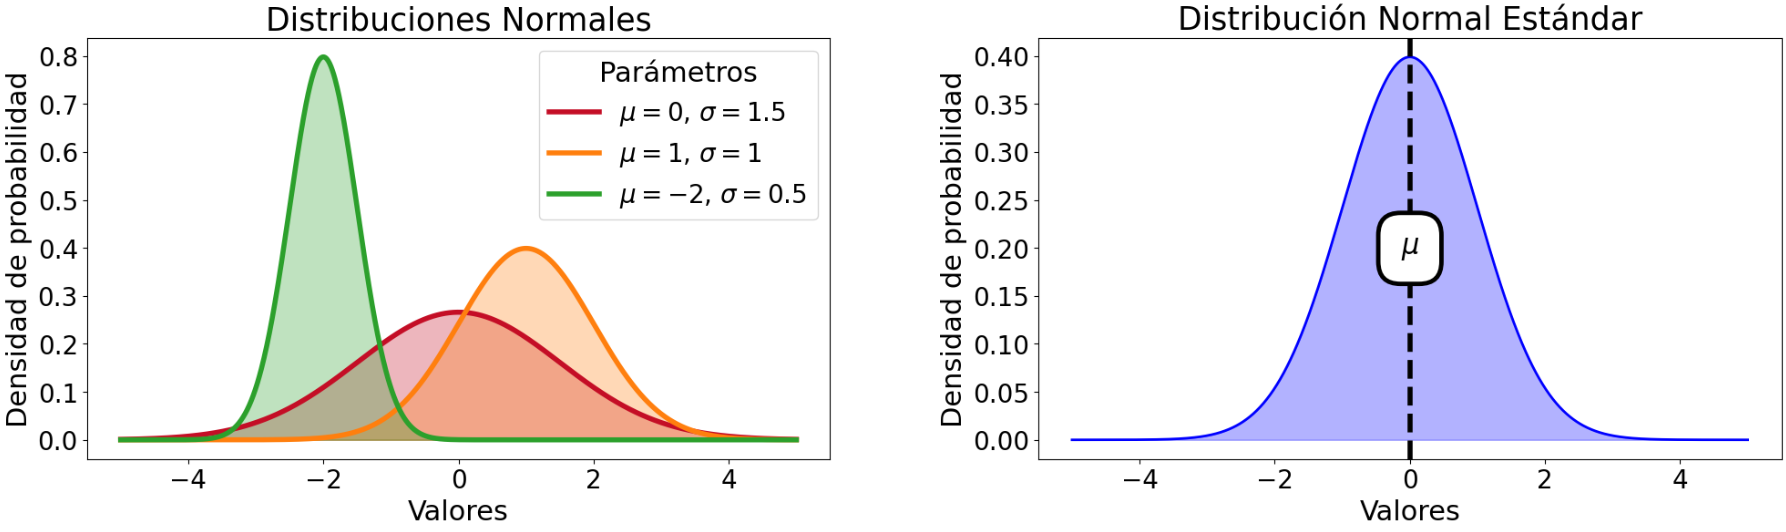
\includegraphics[width=0.8\textwidth]{img/distribuciones-normales.png}
    \caption[Ejemplos de distribuciones normales.] {Ejemplos de distribuciones normales. A la izquierda observamos distintas distribuciones normales, donde podemos notar como el parámetro $\mu$ determina el centro de la distribución y el parámetro $\sigma$ controla la dispersión de los datos. A la derecha observamos una distribución normal estándar, donde se puede apreciar con claridad que la distribución es simétrica con respecto a $\mu$. Imagen original del autor.}\label{fig:distribuciones-normales}
\end{figure}

\chapter{Álgebra Lineal: Matrices}\label{ch:capitulo-algebral-lineal:matrices}

En este capítulo se realizará una introducción al álgebra lineal de matrices, con el objetivo de presentar dos conceptos fundamentales de cara al desarrollo del trabajo: la descomposición en valores singulares y la pseudoinversa de una matriz. Estos conceptos serán presentados de manera precisa y estructurada, proporcionando las bases teóricas necesarias para su comprensión y aplicación en contextos posteriores.\newline

En cuanto a las referencias utilizadas a lo largo de este capítulo, debemos destacar~\cite{Friedberg2014linear}, \cite{Strang2023} y~\cite{Poole2011}. Estos libros nos ayudaron a presentar los conceptos básicos más importantes, así como las demostraciones de los resultados más relevantes del capítulo.

\section{Vectores y espacios vectoriales}\label{sec:vectores-y-espacios-vectoriales}

En primer lugar, se realizará una presentación de los conceptos básicos necesarios, incluyendo los vectores y la estructura de los espacios vectoriales. Estos elementos serán fundamentales para establecer una base sólida para comprender las operaciones y propiedades esenciales en el álgebra lineal de matrices.\newline

\begin{definicion}
    Un cuerpo $F$ es un conjunto en el que dos operaciones $+$ y $\bullet$, llamadas, respectivamente, suma y multiplicación, están definidas de manera que, para cada par de elementos $x, y \in F$, existe únicos elementos $x + y, x \bullet y \in F$ para los que se cumplen las siguientes condiciones para todos los elementos $a, b, c \in F$:

    \begin{enumerate}
        \item $a + b = b + a$ \space y \space $a \bullet b = b \bullet a$.
        \item $(a+b)+c=a+(b+c)$ \space y \space $(a \bullet b) \bullet c=a \bullet (b \bullet c)$.
        \item Existen elementos distintos $0$ y $1$ en $F$ de manera que $0 + a = a$ \space y \space $1 \bullet a = a$.
        \item Para cada elemento $a \in F$ y cada elemento distinto de cero $b \in F$, existen elementos $c, d \in F$ verificando $a+c=0$ \space y \space $b \bullet d = 1$.
        \item $a \bullet (b+c) = a \bullet b + a \bullet c$.
    \end{enumerate}
\end{definicion}

Denominaremos \emph{escalares} a los elementos de un cuerpo $F$. En nuestro caso, centraremos nuestra atención en el cuerpo de los números reales $(\mathbb{R})$ con las definiciones usuales de suma y multiplicación.\newline

\begin{definicion}
    Un objeto de la forma $(a_{1}, a_{2}, \ldots, a_{n})$ cuyas entradas $a_{1}, a_{2}, \ldots, a_{n}$ son elementos de un cuerpo $F$, se denomina una $n$-tupla con entradas o componentes en $F$. Además, dos $n$-tuplas $(a_{1}, a_{2}, \ldots, a_{n})$ y $(b_{1}, b_{2}, \ldots, b_{n})$ cuyas componentes pertenecen al cuerpo $F$ serán iguales si $a_{i} = b_{i}, \; \forall i \in \{1,2, \ldots, n\}$.\newline
\end{definicion}

Una vez expuestas las definiciones de cuerpo y $n$-tupla, podemos introducir el concepto clave de esta sección: el espacio vectorial. A partir de esta noción fundamental, será posible definir de manera precisa el concepto de vector, que será utilizado en la sección siguiente para definir el concepto de matriz.\newline

\begin{definicion}
    Un espacio vectorial $V$ sobre un cuerpo $F$ consiste en un conjunto en el que dos operaciones (denominadas suma y multiplicación por escalar, respectivamente) están definidas de manera que, para cada par de elementos $x, y \in V$ existe un único elemento $x+y \in V$ y para cada elemento $a \in F$ y cada elemento $x \in V$ existe un único elemento $ax \in V$ cumpliendo las siguientes propiedades:

    \begin{enumerate}
        \item $\forall x,y \in V, \; x+y=y+x$.
        \item $\forall x,y,z \in V, \; (x+y)+z=x+(y+z)$.
        \item Existe un elemento en V, denotado por $0$ de manera que $x+0=x, \; \forall x \in V$.
        \item Para cada elemento $x \in V$ existe un elemento $y \in V$ de manera que $x+y=0$.
        \item $\forall x \in V, \; 1x = x$.
        \item Para cada par de elementos $a,b \in F$ y cada elemento $x \in V$, \; $(ab)x = a(bx)$.
        \item Para cada elemento $a \in F$ y cada par de elementos $x,y \in V$, \; $a(x+y) = ax + ay$.
        \item Para cada par de elementos $a,b \in F$ y cada elemento $x \in V$, \; $(a+b)x = ax+bx$.
    \end{enumerate}
\end{definicion}

Denominaremos \emph{vectores} a los elementos, generalmente tuplas de un determinado tamaño, de un espacio vectorial $V$.\newline

\begin{observacion}
    El conjunto de todas las $n$-tuplas con entradas en un cuerpo $F$ se denota por $F^{n}$ (formado por el producto cartesiano de $n$ veces el cuerpo $F$). Este conjunto es un espacio vectorial sobre $F$ con las operaciones de suma y multiplicación por coordenadas. Es decir, sean $u = (u_{1}, u_{2}, \ldots, u_{n}) \in F^{n}$, $v = (v_{1}, v_{2}, \ldots, v_{n}) \in F^{n}$ y $c \in F$, entonces:
    \begin{itemize}
        \item $u + v = (u_{1}+v_{1}, u_{2}+v_{2},\ldots, u_{n}+v_{n})$.
        \item $cu = (cu_{1}, cu_{2}, \ldots, cu_{n})$.
    \end{itemize}

    Además, los vectores de $F^{n}$ se escribirán como vectores columna en lugar de vectores fila. Es decir, si $v \in F^{n}$ entonces

    \[ 
        v = \begin{pmatrix} 
            v_{1} \\ 
            v_{2} \\ 
            \vdots \\
            v_{n}
        \end{pmatrix} = {(v_{1}, v_{2}, \ldots, v_{n})}^{T} 
    \]
        
\end{observacion}

De esta manera, $\mathbb{R}^{n}$ es un espacio vectorial sobre $\mathbb{R}$. Asimismo, dado que nuestro estudio se restringe al cuerpo de los números reales, un vector (real) de dimensión $n$ hará referencia a una $n$-tupla de números reales, es decir $v \in \mathbb{R}^{n}, \; v = {(v_{1}, v_{2}, \ldots, v_{n})}^{T}$, donde $v_{i} \in \mathbb{R}$ para cada $i \in \{1,2, \ldots, n\}$.\newline


Finalmente, se introducen los conceptos de norma y ortonormalidad de vectores, que serán de gran utilidad en el desarrollo de resultados posteriores..

\begin{definicion}
    La \emph{norma (o longitud)} de un vector $v \in \mathbb{R}^{n}$ es el escalar no negativo $||v||$ definido por 

    \[ ||v|| = \sqrt{v \cdot v} = \sqrt{v_{1}^{2}, v_{2}^{2} + \cdots + v_{n}^{2}}. \]\newline
\end{definicion}

\begin{definicion}
    Diremos que dos vectores $u, v \in \mathbb{R}^{n}$ son \emph{ortogonales} si $u \cdot v = 0$. A su vez, diremos que dos vectores $u, v \in V$ son \emph{ortonormales} si son ortogonales y unitarios (su norma es igual a 1).\newline
\end{definicion}

\section{Introducción a las matrices}\label{sec:intro-matrices}

A continuación, se introducirá el concepto de matriz, así como las operaciones y propiedades básicas asociadas a las mismas, que serán las herramientas fundamentales para entender los conceptos clave expuestos en la próxima sección.\newline

\begin{definicion}
    Una matriz $A$ de tamaño $m \times n$ ($m, n \in \mathbb{N}$) con entradas en un cuerpo $F$ es un conjunto bidimensional de la forma 
    
    \[ A =
        \begin{pmatrix} 
        a_{11} & a_{12} & \cdots & a_{1n} \\ 
        a_{21} & a_{22} & \cdots & a_{2n} \\ 
        \vdots & \vdots & \ddots & \vdots \\ 
        a_{m1} & a_{m2} & \cdots & a_{mn} 
        \end{pmatrix}
    \]

    donde cada entrada $a_{ij}$ $(1 \leq i \leq  m, 1 \leq j \leq n)$ es un elemento de $F$. Además, llamamos a las entradas $a_{ij}$ con $i=j$ las entradas diagonales de la matriz. Asimismo, las entradas de la forma $a_{i1}, a_{i2}, \ldots, a_{in}$ forman la $i$-ésima fila de la matriz y las entradas de la forma $a_{1j}, a_{2j}, \ldots, a_{mj}$ forman la $j$-ésima columna de la matriz. De esta manera, las filas de la matriz anterior se consideran vectores ($n$-tuplas) en $F^{n}$ y las columnas se consideran vectores ($m$-tuplas) en $F^{m}$. Finalmente, la matriz cuyas entradas son todas iguales a cero es llamada la matriz cero y se denota por $O$.\newline

\end{definicion}

\begin{definicion}
    Denotaremos por $a_{ij}$ a la entrada de la matriz $A$ correspondiente a la $i$-ésima fila y a la $j$-ésima columna. De esta manera, dadas dos matrices $A$ y $B$ de tamaño $m \times n$, diremos que son \textbf{iguales} si todas sus correspondientes entradas son iguales, es decir, $a_{ij} = b_{ij}$ donde $1 \leq i \leq m$ y $1 \leq j \leq n$.\newline 
\end{definicion}

\begin{observacion}
    El conjunto de todas las matrices de tamaño $m \times n$ con entradas en un cuerpo $F$ es un espacio vectorial que denotaremos por $\mathcal{M}_{m \times n}(F)$ con las operaciones de suma y multiplicación escalar siguientes. Sean $A, B \in \mathcal{M}_{m \times n}(F)$ y $c \in F$, entonces:

    \begin{itemize}
        \item $(a + b)_{ij} = a_{ij} + b_{ij}$ donde $1 \leq i \leq m$ y $1 \leq j \leq n$.
        \item $(ca)_{ij} = ca_{ij}$ donde $1 \leq i \leq m$ y $1 \leq j \leq n$.\newline
    \end{itemize}
\end{observacion}

Una vez conocidas la suma y multiplicación por escalares de matrices, la operación utilizada con más frecuencia es su producto, el cual se definirá a continuación.

\begin{definicion}
    Sea $A$ una matriz de tamaño $m \times n$ y $B$ una matriz de tamaño $n \times p$. Definimos el producto de las matrices $A$ y $B$, denotado por $AB$, como la matriz de tamaño $m \times p$ cuyas entradas se corresponden con

    \[ (ab)_{ij} = \sum_{k=1}^{n} a_{ik}b_{kj}, \quad \text{donde $1 \leq i \leq m$ \space y \space $1 \leq j \leq p$.}\]\newline
\end{definicion}

Seguidamente, se presentan definiciones de algunos tipos de matrices que serán de gran utilidad a lo largo del trabajo.

\begin{definicion}
    Llamaremos matriz \textbf{cuadrada} a toda matriz $A$ con el mismo número de filas y columnas, es decir, $A$ es de la forma $m \times m$ con $m \in \mathbb{N}$ y el espacio vectorial asociado lo denotaremos, simplemente, como $A \in \mathcal{M}_{m}(F)$.\newline
\end{definicion}

\begin{definicion}
    La matriz \textbf{traspuesta} $A^{T}$ de una matriz $A \in \mathcal{M}_{m \times n}(F)$ es la matriz de tamaño $n \times m$ que se obtiene de la matriz $A$ al intercambiar las filas por las columnas, es decir $(a^{T})_{ij} = a_{ji}$. A su vez, decimos que una matriz $A$ es \textbf{simétrica} si cumple $A^{T} = A$. De la propia definición se deduce que una matriz simétrica debe ser cuadrada.\newline
\end{definicion}

\begin{definicion}
    Una matriz cuadrada $A$ de tamaño $n$ se llama \textbf{ortogonal} si sus columnas están formadas por vectores ortonormales dos a dos.\newline
\end{definicion}

Dado que el producto de matrices es una operación no convencional, es necesario identificar el elemento neutro de dicho producto, que se corresponderá con lo que denominaremos como matriz identidad. Su nombre proviene de su relación con la aplicación identidad, dado que representa una función de un espacio vectorial sobre sí mismo.

\begin{definicion}
    Definimos la delta de Kronecker $\delta_{ij}$ como la función dada por

    \[
        \delta_{ij} =
        \begin{cases}
            1 & \text{si } i = j \leq r, \\
            0 & \text{si } i \neq j.
        \end{cases}
    \]

    De esta manera, definimos la \textbf{matriz identidad} de tamaño $n \times n$ ($I_{n}$) como $(i)_{ij} = \delta_{ij}$. Destacamos de la definición que la matriz identidad es una matriz cuadrada y simétrica.\newline
\end{definicion}

\begin{ejemplo}
    A continuación, se presentan las matrices identidad hasta tamaño $n$:
    \[
        I_1 = \begin{pmatrix} 1 \end{pmatrix}, \quad
        I_2 = \begin{pmatrix} 1 & 0 \\ 0 & 1 \end{pmatrix}, \quad
        I_3 = \begin{pmatrix} 1 & 0 & 0 \\ 0 & 1 & 0 \\ 0 & 0 & 1 \end{pmatrix}, \quad \cdots, \quad
        I_n = \begin{pmatrix} 
        1 & 0 & 0 & \cdots & 0 \\ 
        0 & 1 & 0 & \cdots & 0 \\ 
        0 & 0 & 1 & \cdots & 0 \\ 
        \vdots & \vdots & \vdots & \ddots & \vdots \\ 
        0 & 0 & 0 & \cdots & 1 
        \end{pmatrix}
    \]\newline
\end{ejemplo}

\subsection{Rango de una matriz}\label{subsec:rango-matriz}

En esta sección, se abordará el concepto de rango de una matriz, una propiedad fundamental en álgebra lineal, ya que proporciona información crucial sobre la dimensión del espacio generado por sus filas o columnas, y tiene aplicaciones clave en la determinación de la invertibilidad de una matriz.\newline

Comenzaremos con unas definiciones previas, realtivas a los vectores, que nos ayudarán a lo largo de la sección.
\begin{definicion}
    Sea $V$ un espacio vectorial y $S$ un subconjunto no vacío de $V$. Un vector $v \in V$ se dice que es una \textbf{combinación lineal} de vectores de $S$ si existe un número finito de vectores $u_{1}, u_{2}, \ldots, u_{n} \in S$ y escalares $a_{1}, a_{2}, \ldots, a_{n} \in F$ de manera que $v = a_{1}u_{1}, a_{2}u_{2}, \ldots, a_{n}u_{n}$. En este caso, diremos que $v$ es una combinación lineal de $u_{1}, u_{2}, \ldots, u_{n}$ y llamaremos a $a_{1}, a_{2}, \ldots, a_{n}$ los coeficientes de la combinación lineal.\newline 
\end{definicion}

\begin{observacion}
    En cualquier espacio vectorial $V$, el vector cero (todas sus entradas se corresponden con el $0$) es una combinación lineal de cualquier subconjunto no vacío de $V$, dado que $0v = 0$.\newline 
\end{observacion}

\begin{definicion}
    Un subconjunto $S$ de un espacio vectorial $V$ es llamado \textbf{linealmente dependiente} si existe un número finito de vectores distintos $u_{1}, u_{2}, \ldots, u_{n} \in S$ y escalares $a_{1}, a_{2}, \ldots, a_{n}$, donde no todos pueden ser $0$, de manera que

    \[ a_{1}u_{1} + a_{2}u_{2} + \cdots + a_{n}u_{n} = 0. \]

    En este caso, también decimos que los vectores de $S$ son linealmente dependientes.\newline
\end{definicion}

\begin{definicion}
    Un subconjunto $S$ de un espacio vectorial que no es linealmente dependiente es llamado \textbf{linealmente independiente}. De igual manera que en la definición anterior, decimos que los vectores de $S$ son linealmente independientes.\newline
\end{definicion}

\begin{observacion}
    De las definiciones anteriores se extrae que un vector $v \in V$ es linealmente independiente si no puede ser expresado como combinación lineal de otros vectores del espacio (a excepción del vector cero).\newline
\end{observacion}

En lo que sigue, se presentan nuevas definiciones sobre matrices, que serán de utilidad para calcular el rango de una matriz.

\begin{definicion}
    Sea $A$ una matriz de tamaño $m \times n$. Se dice que $A$ es una matriz \textbf{escalonada} si es $O$ o satisface las tres condiciones siguientes:

    \begin{enumerate}
        \item El primer elemento no nulo de cada fila, si existe, es un 1.
        \item El primer 1 de la segunda y sucesivas filas está a la derecha del primer 1 de la fila anterior.
        \item Si tiene filas nulas (compuestas únicamente por ceros), estas aparecen en la parte inferior de la matriz, justo debajo de las filas no nulas.\newline
    \end{enumerate}

    Además, las operaciones elementales que se pueden realizar a una matriz para obtener su forma escalonada son las siguientes:

    \begin{itemize}
        \item Intercambiar dos filas (columnas).
        \item Multiplicar una fila (columna) por un múltiplo distinto de cero.
        \item Sumar un múltiplo de una fila (columna) a otra fila (columna).\newline
    \end{itemize}
\end{definicion}

\begin{definicion}
    Sean $A$ y $B$ dos matrices de tamaño $m \times n$. Se dice que la matriz $A$ es \textbf{equivalente} por filas a la matriz $B$ (o simplemente equivalente) si $B$ se obtiene de $A$ por medio de la aplicación sucesiva de operaciones elementales.\newline
\end{definicion}

\begin{definicion}
    Una matriz $A$ de tamaño $m \times n$ es \textbf{escalonada reducida} si es escalonada y además todo elemento en una columna que esté encima del primer uno de cualquier fila es cero.
\end{definicion}

\begin{ejemplo}
    Para matrices cuadradas de tamaño $2$, las posibles matrices escalonadas reducidas son las siguientes:

    \[
        \begin{pmatrix} 0 & 0 \\ 0 & 0 \end{pmatrix}, \quad
        \begin{pmatrix} 1 & 0 \\ 0 & 1 \end{pmatrix}, \quad
        \begin{pmatrix} 1 & $x$ \\ 0 & 0 \end{pmatrix} \quad y \quad
        \begin{pmatrix} 0 & 1 \\ 0 & 0
        \end{pmatrix}
    \]

    donde $x \in F$ puede ser cualquier escalar.\newline
\end{ejemplo}

Una vez introducidas las definiciones anteriores, disponemos de todas las herramientas necesarias para introducir el concepto de rango de una matriz.

\begin{definicion}[Rango de una matriz]
    Sea $A$ una matriz de tamaño $m \times n$. Se denomina \textbf{rango} de $A$ ($rang(A)$) al número de filas no nulas de la matriz en la forma escalonada reducida equivalente a $A$. De manera equivalente, el rango de una matriz se puede definir como la dimensión del espacio generado por sus vectores fila o columna. De esta manera, el rango de una matriz será igual al número de vectores fila o columna que sean linealmente independientes entre sí.\newline
\end{definicion}

\subsection{Matriz invertible}\label{subsec:matriz-invertible}

En esta sección, se introducirá el concepto de matriz invertible, que se encontrará ampliamente ligado al rango de la matriz. Además, se presentarán algunas propiedades básicas de las matrices invertibles, necesarias para el desarrollo del trabajo.

\begin{definicion}\label{def:matrices-inversas}
    Sea $A$ una matriz cuadrada de tamaño $n$. Entonces la matriz $A$ es \textbf{invertible} (tiene inversa) si existe una matriz $B$ de tamaño $n \times n$ de manera que $AB = BA = I$, donde $I$ denota la matriz identidad de tamaño $n$.\newline
\end{definicion}

\begin{observacion}
    La formulación realizada en la Definición~\ref{def:matrices-inversas} de invertibilidad de matrices sólo es válida para matrices cuadradas.\newline
\end{observacion}

\begin{corolario}\label{cor:inversa-unica}
    Sea $A$ una matriz cuadrada de tamaño $n$. Si $A$ es invertible, entonces la matriz $B$ que verifica $AB = BA = I$ es única. Además, a la matriz B se le denomina la matriz \textbf{inversa} de $A$ y se le denota por $A^{-1}$.
\end{corolario}

\begin{proof}
    Sea $A$ una matriz cuadrada de tamaño $n$ y sean $B$ y $C$ dos matrices verificando $AB = BA = I$ y $AC = CA = I$. Entonces, se verifica

    \[ C = CI = C(AB) = (CA)B = IB = B\]

    donde se ha usado que el producto de matrices es asociativo.\newline
\end{proof}

Tras haber presentado la definición de matriz invertible procedemos a exponer un resultado que nos indicará cuando una matriz admite inversa.

\begin{teorema}
    Sea $A$ una matriz cuadrada de tamaño $n$, entonces equivalen:

    \begin{enumerate}
        \item $A$ es invertible.
        \item $A$ es equivalente a $I_n$.
        \item El rango de $A$ es $n$.
    \end{enumerate}
\end{teorema}

\begin{proof} El teorema quedará probado al demostrar la cadena de implicaciones \textbf{\((1) \implies (2) \implies (3) \implies (1)\)}.\newline

    \textbf{\((1) \implies (2)\)}. Dado que $A$ es invertible, existe $A^{-1}$ verificando $AA^{-1}=I_n$. Además $A^{-1}$ puede expresarse como producto de matrices elementales, es decir, $A^{-1} = E_k \cdots E_2 E_1$. Esto implica que $A$ puede transformarse mediante operaciones elementales de filas a la matriz $I_n$.\newline

    \textbf{\((2) \implies (3)\)}. Si $A$ es equivalente a la matriz $I_n$, significa que mediante operaciones elementales podemos reducir $A$ a la matriz identidad. Por tanto, dado que $I_n$ está formado por $n$ vectores fila linealmente independientes, se deduce que el rango es $n$.\newline

    \textbf{\((3) \implies (1)\)} Sabemos que $A$ es equivalente a su forma escalonada reducida $RA$, donde $R$ es la matriz resultante de multiplicar las distintas operaciones elementales utilizadas, que es invertible al ser producto de matrices elementales. Dado que $rang(A) = n$ todas las filas de la matriz $RA$ son distintas del vector cero y, como $RA$ es una matriz cuadrada en la forma escalonada reducida, se tiene que $RA =I_n$. Como $R$ es invertible, todas las inversas por la izquierda de $R$ son las mismas que las inversas por la derecha de $R$, luego se tiene que $RA = AR = I_n$ y, por tanto, $A$ es invertible con inversa $R$.\newline
\end{proof}

Finalmente, se detallarán algunas de las propiedades más importantes y relevantes a lo largo del desarrollo del trabajo de las matrices invertibles.

\begin{teorema}
    Sean $A$ y $B$ matrices cuadradas e invertibles del mismo tamaño. Entonces se cumple:

    \begin{enumerate}
        \item $A^{-1}$ es invertible y ${(A^{-1})}^{-1} = A$ (la inversa de $A^{-1}$ es la propia matriz $A$).
        \item $A^{T}$ es invertible y ${(A^{T})}^{-1} = {(A^{-1})}^{T}$.
        \item La matriz $AB$ es invertible y ${(AB)}^{-1} = B^{-1}A^{-1}$.
    \end{enumerate}
\end{teorema}

\begin{proof}
    \textbf{\((1)\)}. Dado que $A$ es invertible, se verifica que $A^{-1}A = AA^{-1} = I$, luego también $A^{-1}$ es invertible y su inversa (que sabemos que es única por el Corolario~\ref{cor:inversa-unica}) es la propia matriz $A$.\newline

    \textbf{\((2)\)}. Sabemos que la matriz $A$ es invertible, luego verifica $A^{-1}A = AA^{-1} = I$. Tomamos ahora la traspuesta en ambos lados de la ecuación, obteniendo ${(A^{-1}A)}^{T} = {(AA^{-1})}^{T} = I^{T}$. Usando que la traspuesta de un producto de matrices es ${(AB)}^{T} = B^{T}A^{T}$, obtenemos el resultado deseado.\newline

    \textbf{\((3)\)}. Basta comprobar que ${(AB)B^{-1}A^{-1}} = A(BB^{-1})A^{-1} = AIA^{-1} = AA^{-1} = I$ y que $B^{-1}A^{-1}(AB) = B^{-1}(A^{-1}A)B = B^{-1}IB = B^{-1}B = I$, donde se utiliza que $A$ y $B$ son matrices invertibles y la asociatividad del producto de matrices. \newline
\end{proof}

\section{Determinantes, vectores propios y valores propios}\label{sec:determinante-vectores-valores-propios}

\begin{definicion}
    Sea $A$ una matriz cuadrada de tamaño $n$ con $n \geq 2$. Definimos el \textbf{determinante} de la matriz $A$ ($\det(A)$) como el escalar dado por la función $\det: \mathcal{M}_{n \times n}(F) \to F$, definida como sigue

    \[ \det(A) = a_{11} \det(A_{11}) -  a_{12} \det(A_{12}) + \cdots + (-1)^{n+1}a_{1n} \det(A_{1n}) = \sum_{j=1}^{n}(-1)^{j+1}a_{1j} \det(A_{1j})\]

    donde $A_{ij}$ hace referencia a la submatriz que se obtiene al eliminar de la matriz $A$ la fila $i$-ésima y la columna $j$-ésima. Para el caso $n=1$, el determinante de $A$ es la propia entrada de la matriz $A$.\newline
\end{definicion}


El siguiente resultado nos ayuda a conocer cuando una matriz es invertible a través de su determinante, sin necesidad de tener que encontrar la matriz escalonada reducida.
\begin{corolario}\label{cor:det-inversa}
    Una matriz $A \in \mathcal{M}_{n}(F)$ es invertible si y solo si $\det(A) \neq 0$. Además, si $A$ es invertible, entonces $\det(A^{-1})=\frac{1}{\det(A)}$.
\end{corolario}

\begin{proof}
    Si $A \in \mathcal{M}_{n}(F)$ no es invertible, entonces $rang(A)$ es menor a $n$. Esto significa que $A$ tiene filas (o columnas) que son linealmente dependientes entre sí y, a través de operaciones elementales, podemos obtener una matriz $B$ equivalente a la matriz $A$ con alguna de sus filas formada por un vector nulo, lo que implica que $\det(B) = 0$, pero como $A$ es equivalente a $B$, se verifica que $\det(A) = \det(B) = 0$.\newline

    Por otra parte, si $A \in \mathcal{M}_{n}(F)$ es invertible, entonces se cumple

    \[ \det(A)\cdot\det(A^{-1}) = \det(AA^{-1}) = \det(I_n)=1\]

    donde se hace uso de la propiedad de que el producto de determinantes de matrices cuadradas es igual al determinante del producto de las propias matrices.\newline
\end{proof}

\begin{definicion}
    Sea $A$ una matriz cuadrada de tamaño $n$. Un vector no nulo $v \in F^{n}$ se dice que es un \textbf{vector propio} (o autovector) de la matriz $A$ si $Av=\lambda v$ para algún escalar $\lambda \in F$. Además, el escalar $\lambda$ se llama \textbf{valor propio} (o autovalor) de la matriz $A$ correspondiente al vector propio $v$.\newline
\end{definicion}

El siguiente teorema nos proporciona cómo calcular, de manera práctica, los valores propios de una determinada matriz.
\begin{teorema}
    Sea $A \in \mathcal{M}_{n}(F)$. Entonces un escalar $\lambda \in F$ es un valor propio de la matriz $A$ si y solo si $\det(A - \lambda I_n) = 0$. 
\end{teorema}

\begin{proof}
    Un escalar $\lambda$ es un valor propio de una matriz $A$ si y solo si existe un vector no nulo $v \in F^{n}$ de manera que $Av = \lambda v$, es decir, $(A - \lambda I_n)(v) = 0$. Esto es cierto si y solo si la matriz $A - \lambda I_n$ no es invertible. Sin embargo, este resultado es equivalente (haciendo uso del Corolario~\ref{cor:det-inversa}) al hecho de que $\det(A - \lambda I_n) = 0$.\newline
\end{proof}


\begin{corolario}\label{cor:valores-singulares-positivos}
    Para cualquier matriz $A \in \mathcal{M}_{m \times n}(\mathbb{R})$, la matriz $A^{T}A$ es simétrica y, en consecuencia, puede ser diagonalizable ortogonalmente (teorema espectral real~\cite{Blum2021}). De esta forma, todos los valores propios de la matriz $A^{T}A$ son no negativos.
\end{corolario}

\begin{proof}
    Sea $\lambda$ un valor propio de la matriz $A^{T}A$ con su correspondiente vector propio unitario $v$ asociado. Entonces, se verifica

    \[ 0 \leq ||Av||^{2} = (Av)\cdot(Av)=(Av)^{T}Av=v^{T}A^{T}Av \\ 
     = v^{T}\lambda v = \lambda (v \cdot v) = \lambda ||v||^2 = \lambda.\]\newline
\end{proof}

\section{Descomposición en valores singulares y pseudoinversa}\label{sec:svd-pseudoinversa}
En esta sección se presentan los principales resultados sobre matrices abordados en este trabajo: la descomposición en valores singulares y la pseudoinversa. Cabe destacar que estos resultados se enuncian para matrices con escalares en el cuerpo $\mathcal{R}$, aunque su generalización a otros cuerpos es posible.\newline

\begin{definicion}
    Si $A$ es una matriz de tamaño $m \times n$, los \textbf{valores singulares} de $A$ son las raíces cuadradas (positivas) de los valores propios de la matriz $A^{T}A$ y se denotan mediante $\sigma_{1}, \sigma_{2}, \ldots, \sigma_{n}$. Además, es convencional ordenar los valores singulares de manera que $\sigma_{1} \geq \sigma_{2} \geq \cdots \geq \sigma_{n}$.\newline
\end{definicion}

\begin{observacion}
    Tiene sentido hablar de las raíces cuadradas positivas de los valores propios de la matriz $A^{T}A$ por el resultado obtenido en el Corolario~\ref{cor:valores-singulares-positivos}.\newline
\end{observacion}

El siguiente resultado nos indica que toda matriz, independientemente de su estructura, puede ser factorizada como producto de tres matrices, dos de las cuales serán ortogonales. Este resultado se conoce como \emph{descomposición en valores singulares} y es una de las factorizaciones más importantes de todas las matrices.
\begin{teorema}[Descomposición en valores singulares]
    Sea $A \in \mathcal{M}_{m \times n}(\mathbb{R})$ una matriz cuyo rango es $r$ y con valores singulares positivos $\sigma_{1} \geq \sigma_{2} \geq \cdots \geq \sigma_{r}$ y sea $\Sigma$ la matriz de tamaño $m \times n$ definida por 

    \[
        \Sigma_{ij} =
        \begin{cases}
            \sigma_i & \text{si } i = j \leq r, \\
            0 & \text{en otro caso.}
        \end{cases}
    \]

    Entonces existen una matriz ortogonal de tamaño $m \times m$ $U$ y una matriz ortogonal de tamaño $n \times n$ $V$ de manera que

    \[
        A = U \Sigma V^{T}.
    \]

    A esta factorización la llamaremos \emph{descomposición en valores singulares (SVD)} de $A$.\newline
\end{teorema}

\begin{proof}
    La demostración se fundamenta en la construcción directa de las matrices $V$ y $U$, verificando posteriormente que se satisface el resultado buscado.\newline

    Para construir la matriz ortogonal $V$, hay que encontrar una base ortonormal $\{v_1, v_2, \ldots, v_n \}$ de $F^{n}$ formada por vectores propios de la matriz simétrica y cuadrada $A^{T}A$ de tamaño $n$. Entonces se tiene que $V = [v_1, v_2, \ldots, v_n]$ es una matriz ortogonal y cuadrada de tamaño $n$.\newline

    Para construir la matriz ortogonal $U$, primero notemos que $\{Av_1, Av_2, \ldots, Av_n \}$ es un conjunto ortogonal de vectores de $F^{m}$. Para demostrar esto, basta suponer que $v_i$ es el vector propio de la matriz $A^{T}A$ correspondiente al valor propio $\lambda_i$. Entonces, para $i \neq j$, se cumple

    \[ (Av_i)\cdot(Av_j) = (Av_i)^{T}Av_j=v_{i}^{T}A^{T}Av_j = v_{i}^{T}\lambda_j v_j=\lambda_j(v_i \cdot v_j) = 0\]

    dado que los vectores propios $v_i$ son ortogonales. Recordamos ahora que los valores singulares satisfacen $\sigma_i = ||Av_i||$ y que los primeros $r$ valores singulares son distintos de cero. Por tanto, podemos normalizar $Av_1, \ldots, Av_r$ de la siugiente forma

    \begin{equation}
        u_i = \frac{1}{\sigma_i} A v_i \quad \text{para } i = 1, \ldots, r.
        \label{eq:singulares1}
    \end{equation}
    

    Esto garantiza que $\{ u_1, \ldots, u_r\}$ es un conjunto ortonormal de $F^{m}$, pero si $r < m$ no será una base para $F^{m}$. En este caso, se extiende el conjunto $\{u_1, \ldots, u_r \}$ a una base ortonormal $\{u_1, \ldots, u_m \}$ para $F^{m}$. Entonces se tiene $U = [u_1, u_2, \ldots, u_m]$. Ahora, falta comprobar que, con la construcción realizada, se satisface el resultado $A = U \Sigma V^{T}$. Dado que $V^{T} = V^{-1}$ (al ser la matriz $V$ ortogonal), esto equivale a demostrar que $AV = U\Sigma$.\newline

    En primer lugar, sabemos, a partir de la Ecuación~\eqref{eq:singulares1}, que $Av_i=\sigma_i u_i$ para $i=1, \ldots, r$ y que $||A v_i|| = \sigma_i = 0$ para $i=r+1, \ldots,n$. En consecuencia, $Av_i = 0$ para $i=r+1, \ldots,n$. Por tanto, \newline

    \begin{align*}
        A V &= A \begin{bmatrix} \mathbf{v}_1 & \cdots & \mathbf{v}_n \end{bmatrix} \\
            &= \begin{bmatrix} A \mathbf{v}_1 & \cdots & A \mathbf{v}_n \end{bmatrix} \\
            &= \begin{bmatrix} A \mathbf{v}_1 & \cdots & A \mathbf{v}_r & 0 & \cdots & 0 \end{bmatrix} \\
            &= \begin{bmatrix} \sigma_1 \mathbf{u}_1 & \cdots & \sigma_r \mathbf{u}_r & 0 & \cdots & 0 \end{bmatrix} \\
            &= \begin{bmatrix} \mathbf{u}_1 & \cdots & \mathbf{u}_m \end{bmatrix}
               \begin{bmatrix} 
                   \sigma_1 & \cdots & 0 & O \\
                   \vdots & \ddots & \vdots & O \\
                   0 & \cdots & \sigma_r & O \\
                   O & O & O & O
               \end{bmatrix} \\
            &= U \Sigma
    \end{align*}

    quedando probada la igualdad $AV = U \Sigma$.\newline
\end{proof}

Conocemos, de la Subsección~\ref{subsec:matriz-invertible}, cuando una matriz era invertible. Sin embargo, el resultado mostrado únicamente era válido para matrices cuadradas. El siguiente resultado generaliza el concepto de matriz inversa cuando la matriz no es cuadrada.
\begin{definicion}[Pseudoinversa]
    Sea $A \in \mathcal{M}_{m \times n}(\mathbb{R})$ con $m > n$ y donde las columnas de $A$ son linealmente independientes. Se define la \textbf{pseudoinversa} \emph{(o inversa de Moore-Penrose)} de la matriz $A$ como la matriz $A^{\dagger}$ dada por

    \[ A^{\dagger} = {(A^{T}A)}^{-1}A^{T} \]

    donde se puede comprobar que $A^{\dagger} \in \mathcal{M}_{n \times m}(\mathbb{R})$.\newline
\end{definicion}

No obstante, dado que toda matriz se puede factorizar en su descomposición en valores singulares, podemos definir la pseudoinversa de una matriz a partir de dicha factorización.
\begin{definicion}
    Sea $A$ una matriz de tamaño $m \times n$ de rango $r$ con descomposición en valores singulares $A = U \Sigma V^{T}$ y con valores singulares distintos de cero $\sigma_{1} \geq \sigma_{2} \geq \cdots \geq \sigma_{r}$. Sea $\Sigma^{\dagger}$ la matriz de tamaño $n \times m$ definida por

    \[
        \Sigma^{\dagger}_{ij} =
        \begin{cases}
            \frac{1}{\sigma_i} & \text{si } i = j \leq r, \\
            0 & \text{en otro caso.}
        \end{cases}
    \]

    Entonces la factorización $A^{\dagger} = V \Sigma^{\dagger} U^{T}$ es una descomposición en valores singulares de $A^{\dagger}$, donde $\Sigma^{\dagger}$ es la pseudoinversa de $\Sigma$. Además, $A^{\dagger}$ es la pseudoinversa de $A$.\newline
\end{definicion}

El siguiente resultado presenta una forma análoga de definir la pseudoinversa de una matriz, basándose en las propiedades que debe cumplir la pseudoinversa, que serán de gran utilidad en el desarrollo del trabajo.
\begin{definicion}[Condiciones de Moore-Penrose]
    Sea $A \in \mathcal{M}_{m \times n}(\mathbb{R})$, la pseudoinversa de $A$, $A^{\dagger} \in \mathcal{M}_{n \times m}(\mathbb{R})$, es la única matriz que satisface las siguientes propiedades, conocidas como las condiciones de Moore-Penrose:

    \begin{enumerate}
        \item $A A^{\dagger} A = A$.
        \item $A^{\dagger} A A^{\dagger} = A^{\dagger}$.
        \item ${(A A^{\dagger})}^{T}$ es simétrica, es decir, ${(A A^{\dagger})}^{T} = A A^{\dagger}$.
        \item ${(A^{\dagger} A)}^{T}$ es simétrica, es decir, ${(A^{\dagger} A)}^{T} = A^{\dagger} A$.
    \end{enumerate}

    Además, si $A$ es de rango completo, es decir, $rango(A) = r  = \min\{m, n\}$, entonces $A^{\dagger}$ puede expresarse de forma sencilla como sigue

    \begin{itemize}
        \item Si $r = m = n$, entonces la matriz $A$ es invertible y $A^{\dagger} = A^{-1}$.
        \item Si $r = m < n$, entonces $A$ tiene filas linealmente independientes ($A$ es sobreyectiva y $AA^{T}$ es invertible) y $A^{\dagger} = A^{T}{(AA^{T})}^{-1}$.
        \item Si $r = n < m$, entonces $A$ tiene columnas linealmente independientes ($A$ es inyectiva y $A^{T}A$ es invertible) y $A^{\dagger} = {(A^{T}A)}^{-1} A^{T}$.\newline
    \end{itemize}
\end{definicion}

Finalmente, la solución de norma mínima para un problema de mínimos cuadrados puede definirse mediante la pseudoinversa de una matriz, como se establece en el siguiente teorema.

\begin{teorema}
    El problema de mínimos cuadrados $A\mathbf{x}=\mathbf{b}$, con $A \in \mathcal{M}_{m \times n}(\mathbb{R})$, $\mathbf{x} \in \mathbb{R}^{n}$ y $\mathbf{b} \in \mathbb{R}^{m}$, tiene una solución única $\bar{x}$ de mínimos cuadrados de norma mínima dada por

    \[ \bar{\mathbf{x}} = A^{\dagger}\mathbf{b} \]
\end{teorema}

\begin{proof}
    Sea $A \in \mathcal{M}_{m \times n}(\mathbb{R})$ con $rang(A) = r$ y sea $U\Sigma V^{T}$ su descomposición en valores singulares. De este modo, se tiene que $A^{\dagger} = V \Sigma^{\dagger} U^{T}$. Sean $\mathbf{y}=V^{T}\mathbf{x}$ y $\mathbf{c}=U^{T}\mathbf{b}$, expresados de la siguiente forma

    \[
        \mathbf{y} = \begin{bmatrix} \mathbf{y}_1 \\ \mathbf{y}_2 \end{bmatrix}, \quad 
        \mathbf{c} = \begin{bmatrix} \mathbf{c}_1 \\ \mathbf{c}_2 \end{bmatrix}
    \]

    donde $\mathbf{y_1}, \mathbf{c_1} \in \mathbb{R}^{r}$.\newline

    Se busca minimizar $\|\mathbf{b} - A \mathbf{x}\|$ o, de manera equivalente, $\|\mathbf{b} - A \mathbf{x}\|^2$. Usando que $U^T$ es ortogonal (dado que $U$ es ortogonal), se tiene  

    \[
        \|\mathbf{b} - A \mathbf{x}\|^2 = \| U^T (\mathbf{b} - A \mathbf{x}) \|^2 = \| U^T (\mathbf{b} - U \Sigma V^T \mathbf{x}) \|^2 = \| U^T \mathbf{b} - U^T U \Sigma V^T \mathbf{x} \|^2
    \]

    \[
        = \|\mathbf{c} - \Sigma \mathbf{y}\|^2 = \left\| \begin{bmatrix} \mathbf{c}_1 \\ \mathbf{c}_2 \end{bmatrix} - \begin{bmatrix} D & O \\ O & O \end{bmatrix} \begin{bmatrix} \mathbf{y}_1 \\ \mathbf{y}_2 \end{bmatrix} \right\|^2 = \left\| \begin{bmatrix} \mathbf{c}_1 - D \mathbf{y}_1 \\ \mathbf{c}_2 \end{bmatrix} \right\|^2.
    \]\newline

    Dado que sólo disponemos de control sobre $\mathbf{y}_1$, el valor mínimo ocurre cuando $\mathbf{c}_1 - D \mathbf{y}_1 = 0$ o, de manera equivalente, cuando $\mathbf{y}_1 = D^{-1} \mathbf{c}_1$. De modo que todas las soluciones $\mathbf{x}$ de mínimos cuadrados son de la forma  

    \[
        \mathbf{x} = V \mathbf{y} = V \begin{bmatrix} D^{-1} \mathbf{c}_1 \\ \mathbf{y}_2 \end{bmatrix}
    \]

    Definimos $\bar{\mathbf{x}} = V \bar{\mathbf{y}} = V \begin{bmatrix} D^{-1} \mathbf{c}_1 \\ 0 \end{bmatrix}$ y afirmamos que $\bar{\mathbf{x}}$ es la solución de mínimos cuadrados de norma mínima. Para demostrarlo, supongamos que $\mathbf{x}^{\prime}=V\mathbf{y}^{\prime} = V \begin{bmatrix} D^{-1} \mathbf{c}_1 \\ y_2 \end{bmatrix}$ es otra solución diferente al problema de mínimos cuadrados (por tanto, $\mathbf{y}_2 \neq 0$). Entonces, se verifica

    \[ \| \bar{\mathbf{x}} \| = \| V\bar{\mathbf{y}} \| = \| \bar{\mathbf{y}} \| < \| {\mathbf{y}^{\prime}} \| = \| V\mathbf{y}^{\prime} \| = \| \mathbf{x}^{\prime} \|\]

    como se quería probar. Por último, falta demostrar que $\bar{\mathbf{x}}$ es igual a $A^{\dagger}\mathbf{b}$. Para ello, basta calcular

    \[ \bar{\mathbf{x}} = V\bar{\mathbf{y}} = V \begin{bmatrix} D^{-1} \mathbf{c}_1 \\ 0 \end{bmatrix} = V \begin{bmatrix} D^{-1} & O \\ O & O \end{bmatrix} \begin{bmatrix} \mathbf{c}_1 \\ \mathbf{c}_2 \end{bmatrix} = V \Sigma^{\dagger} \mathbf{c} = V \Sigma^{\dagger} U^{T} \mathbf{b} = A^{\dagger}\mathbf{b}.\]

    
\end{proof}

% \chapter{Aproximación lineal}\label{ch:capitulo-aproximacion-lineal}

\endinput